\documentclass[xcolor=svgnames,aspectratio=169]{beamer} 
\usetheme{metropolis}
\usefonttheme{professionalfonts}
\setbeamertemplate{theorems}[numbered]
\usepackage{luatexja}
\usepackage{luatexja-fontspec}
\usepackage{newtxtext}                     
\usepackage{amsthm} 
\usepackage{graphicx}
\usepackage{xcolor}
\usepackage{tcolorbox}
\usepackage{tikz}
\everymath{\displaystyle}
\usepackage{bbm}
\usepackage{lmodern}
\newcommand{\indep}{\mathop{\perp\!\!\!\!\perp}}
\newcommand{\R}{\mathbb{R}} 
\newcommand{\N}{\mathbb{N}} 
\newcommand{\Z}{\mathbb{Z}} 
\newcommand{\Q}{\mathbb{Q}} 
\newcommand{\C}{\mathbb{C}}
\newcommand{\E}{\mathbb{E}}

\begin{document} 

\title{Matrix Completion Methods for Causal Panel Data Models \\ \small{Susan Athey et al. (2021), JASA}}
\author{Naoki Eguchi}          
\institute{Faculty of Medicine, Kyoto University} 
\date{\today}

\begin{frame}                  
    \titlepage                     
\end{frame}

\section{Introduction}

\begin{frame}{Today's Agenda ; Keyword : Imputation}
    \begin{itemize}
        \item
    \end{itemize}
\end{frame}

\begin{frame}{Imputation}
    \begin{itemize}
        \item As many panel data methods, we want to know ATT : $\E[Y_{it}(1)-Y_{it}(0)|W_i=1]$.
        \item Thus, it boils down to estimate (impute) the counterfactual $Y_{it}(0)$.
        \begin{itemize}
            \item Horizontal : Under unconfoundedness, we can impute counterfactual PO using observed outcomes for control units.
            \item Vertical : By SCM, we can also impute it using weighted average outcomes for control units with most predictive weights trained with pre-treatment datas.
        \end{itemize}
        \begin{figure}
            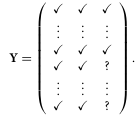
\includegraphics[width=0.5\textwidth, height=0.4\textheight, keepaspectratio]{Horizontal.png} \ 
            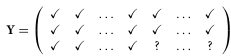
\includegraphics[width=0.5\textwidth, height=0.5\textheight, keepaspectratio]{Vertical.png}
        \end{figure}
    \end{itemize}
\end{frame}

\begin{frame}{Xu (2024): Counterfactual estimation}
    \begin{itemize}
        \item functional form: 
        $
        Y_{it}(0)=f(\mathbf{X_{it}})+h(\mathbf{U_{it}})+\epsilon_{it}
        $ \\
        \rightarrow No anticipation, carryover, feedback, LDV
        \item strict exogeneity:
        $
        \forall i,j\in\{1,\dots,N\},\ \forall s,t\in\{1,\dots,T\}, \epsilon_{it}\ \indep\ \{D_{js}, \mathbf{X_{js}}, \mathbf{U_{js}}\}
        $
        \begin{figure}
            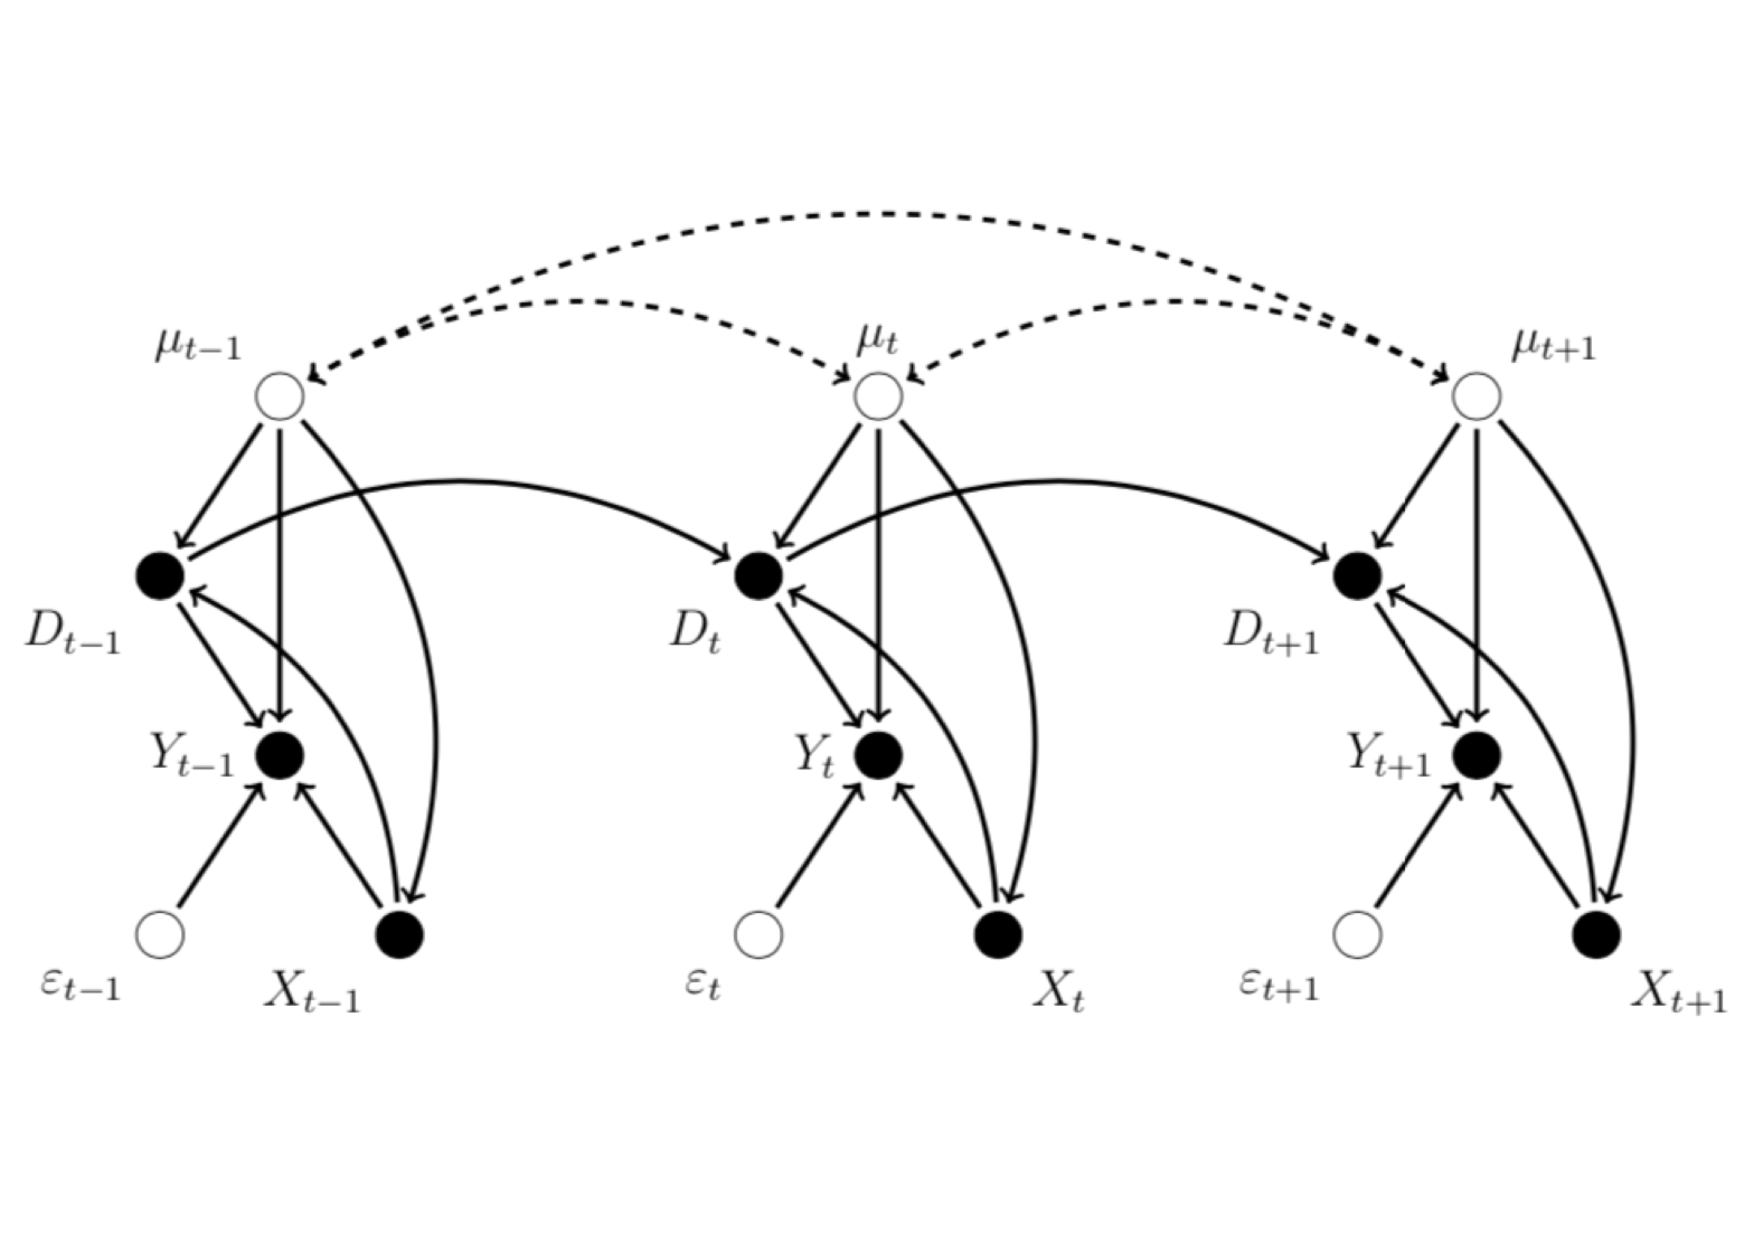
\includegraphics[width=\textwidth, height=0.4\textheight, keepaspectratio]{Xu_DAG.pdf}
        \end{figure}
        \item low-dimensional decomposition:
        $
        h(\mathbf{U_{it}})=\{L_{it}\}, \mathrm{rank}(\mathbf{L}_{N\times T}) \ll \min\{N,T\}
        $

        →The rank (= number of factors) is \alert{FIXED !!}
    \end{itemize}
\end{frame}

\section{Set Up}

\begin{frame}{Notation and Estimand}
    \begin{itemize}
        \item Consider a setting with $N$ units observed over $T$ periods characterized by a binary treatment $W_{it}$ and hence two POs $Y_{it}(1), Y_{it}(0)$.
        \begin{itemize}
            \item $\mathbf{X}\in\R^{N\times P} \ , \  \mathbf{Z}\in\R^{T\times Q}$ : observe (unit / time)-specific covariance matrix
        \end{itemize}
        \item Estimand : $\mathbf{Y} = \{Y_{it}(0)\footnote{以降は簡単のため,$Y_{it}(0)=Y_{it}$ とし,“(0)” を省略して表記する.}\}
        =
        \begin{pmatrix}
Y_{11}(0) & \cdots & Y_{1T}(0) \\
\vdots & \ddots & \vdots \\
Y_{N1}(0) & \cdots & Y_{NT}(0)
\end{pmatrix}$ (← Matrix!!)
        \item $W_{it}=
        \begin{cases}
            1 & \text{if} \ (i,t)\in \mathcal{M} \\ 0 & \text{if} \ (i,t) \in\mathcal{O} 
        \end{cases}$
    \end{itemize}
\end{frame}

\begin{frame}{Patterns of data matrix}
    \begin{itemize}
        \item Ordinary case (rich data wrt. units and times)
        \begin{figure}
            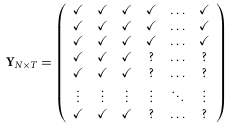
\includegraphics[width=\textwidth, height=0.35\textheight, keepaspectratio]{Ordinary.png}
        \end{figure}
        \item Staggered adoption
        \begin{figure}
            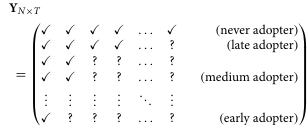
\includegraphics[width=\textwidth, height=0.35\textheight, keepaspectratio]{Staggered_adoption.png}
        \end{figure}
    \end{itemize}
\end{frame}

\begin{frame}{Horizontal regression and unconfoundedness : thin matrix ($N\gg T$)}
    \begin{figure}
            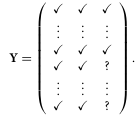
\includegraphics[width=0.5\textwidth, height=0.4\textheight, keepaspectratio]{Horizontal.png} 
        \end{figure}
    \begin{enumerate}
        \item Regress the last period outcome on the lagged outcomes. (among untreated)
        \item Predict the missing POs using the estimated regression.
        \[
        \forall (i,T)\in\mathcal{M} , \ \hat{Y}_{iT}=\hat{\beta}_0+\sum_{t=1}^{T-1}\hat{\beta}_tY_{it}, \ \text{where} \ \ \hat{\beta}=\arg\min_{\beta} \sum_{i:(i,T) \in \mathcal{O} }(Y_{iT}-\beta_0-\sum_{t=1}^{T-1}\beta_tY_{it})^2.
        \]
    \end{enumerate}
    →Nonparametrically, 
\end{frame}

\begin{frame}{Vertical regression and synthesis control : fat matrix ($T\gg N$)}
    \begin{figure}
            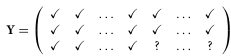
\includegraphics[width=0.5\textwidth, height=0.5\textheight, keepaspectratio]{Vertical.png}
    \end{figure}
    \begin{enumerate}
        \item Regress the outcomes for treated unit prior to the treatment on the outcomes for the control units in the same periods.
        \item Predct the missing POs using the estimated regression.
        \[
        \forall (N,t)\in\mathcal{M} , \ \hat{Y}_{Nt}=\hat{\gamma}_0+\sum_{i=1}^{N-1}\hat{\gamma}_iY_{it}, \ \text{where} \ \ \hat{\gamma}=\arg\min_{\gamma} \sum_{t:(N,t) \in \mathcal{O} }(Y_{Nt}-\gamma_0-\sum_{i=1}^{N-1}\gamma_iY_{it})^2.
        \]
    \end{enumerate}
    →Vertical regression is generalization of ADH(2010) in that it relaxes two restrictions :
    \begin{itemize}
        \item the coefficients $\hat{\gamma}$ are nonnegative. (Interpretability ; What is a negative weight?)
        \item the intercept in this regression is $0$. (This is seen to be plausible in recent literatures.)
    \end{itemize}
\end{frame}

\section{Matrix Completion}

\begin{frame}{Model}
    \begin{itemize}
        \item Under no covariates, we model the $N\times T$ matrix of complete matrix $\mathbf{Y}$ as
        \[
        \mathbf{Y}=\mathbf{L^*}+\mathbf{\epsilon}, \ \text{where} \ \ \E[\mathbf{\epsilon}|\mathbf{L^*}]=0.
        \]
    \begin{tcolorbox}[colframe=lightgray,title=Assumption 1]
        \begin{itemize}
            \item $\mathbf{\epsilon}$ is independent of $\mathbf{L^*}$
            \item The element of $\mathbf{\epsilon}$ are $\sigma-sub-Gaussian$ and independent each other.
            $\Leftrightarrow \forall t, \ \E[\exp (t\epsilon)]\leq \exp (\frac{\sigma^2t^2}{2}).$
        \end{itemize}
    \end{tcolorbox}
        \item The goal is to estimate the matrix $\mathbf{L^*}$. (low-rank assumption) 
    
        →Note that two types\footnote{Interactive fixed effectも低ランクとしていいが, rankが明示的でないため具体的には考えない.} of fixed effects are included.
    \end{itemize}
\end{frame}

\begin{frame}{}
    \begin{itemize}
        \item 
    \end{itemize}
\end{frame}

\section{Theoritical Bounds \\ for the Estimation Error}

\section{Two illustrations}

\section{References}

\begin{frame}{References}
    \begin{itemize}
        \item Susan Athey, Mohsen Bayati, Nikolay Doudchenko, Guido Imbens, and Khashayar Khosravi (2021), \textit{Matrix Completion Methods for Causal Panel Data Models}, Journal of the American Statistical Association.
        \item Licheng Liu, Ye Wang, Yiqing Xu (2024), \textit{A Practical Guide to Counterfactual Estimators for Causal Inference with Time-Series Cross-Sectional Data},  American Journal of Political Science.
        \item Martin J. Wainwright (2019), \textit{High-Dimensional Statistics}, Cambridge University Press. (mainly Chapter 10)
        \item 冨岡亮太 (2015), スパース性に基づく機械学習, 講談社.
        \item 川口康平,澤田真行 (2024), 因果推論の計量経済学,日本評論社.
    \end{itemize}
\end{frame}

\end{document}